\documentclass{beamer}

\usepackage[utf8]{inputenc}
\usepackage{lmodern}
\usepackage{hyperref}
\usepackage{graphicx}
\usepackage{minted}
\usepackage{epstopdf}
\usepackage{tabularx}
\usepackage{ulem}

\title{Chatbot bouwen}
\subtitle{Zeeslag }
\author{Robin Sikkens \& Maarten van den Berg}
\date{12 december 2017}

\usetheme{Frankfurt}
\usecolortheme{dove}

\setbeamertemplate{section in toc}{\inserttocsectionnumber.~\inserttocsection}
\setbeamertemplate{itemize items}[default]
\setbeamertemplate{enumerate items}[default]

% ToC invoegen aan het begin van elke sectie.
\AtBeginSection
{
  \begin{frame}
      \tableofcontents[currentsection,hideallsubsections,subsubsectionstyle=hide]
    \end{frame}
}
% Bron: https://en.wikibooks.org/wiki/LaTeX/Presentations

\definecolor{light-gray}{gray}{0.90}

\begin{document}
\begin{frame}
	\titlepage
\end{frame}

\section{Wat gaan we doen?}
\begin{frame}{Wat gaan we doen}
	Chatbot bouwen voor Zeeslag (Battleships) tegen computer

	\begin{itemize}
		\item Bepalen hoe een bord op te bouwen
		\item Bepalen hoe ergens op te schieten
	\end{itemize}
\end{frame}

\begin{frame}{Zeeslag}
	\begin{columns}
		\begin{column}{0.5\textwidth}
			\begin{itemize}
				\item 2 speelborden, $10 \times 10$
				\item X: \texttt{A-J}, Y: getal
				\item Schepen:
					\begin{enumerate}
						\item Vliegdekschip (5)
						\item Slagschepen (4)
						\item Onderzeeër (3)
						\item Patrouilleschip (2)
					\end{enumerate}
				\item Om beurten schieten
			\end{itemize}
		\end{column}
		\begin{column}{0.5\textwidth}
			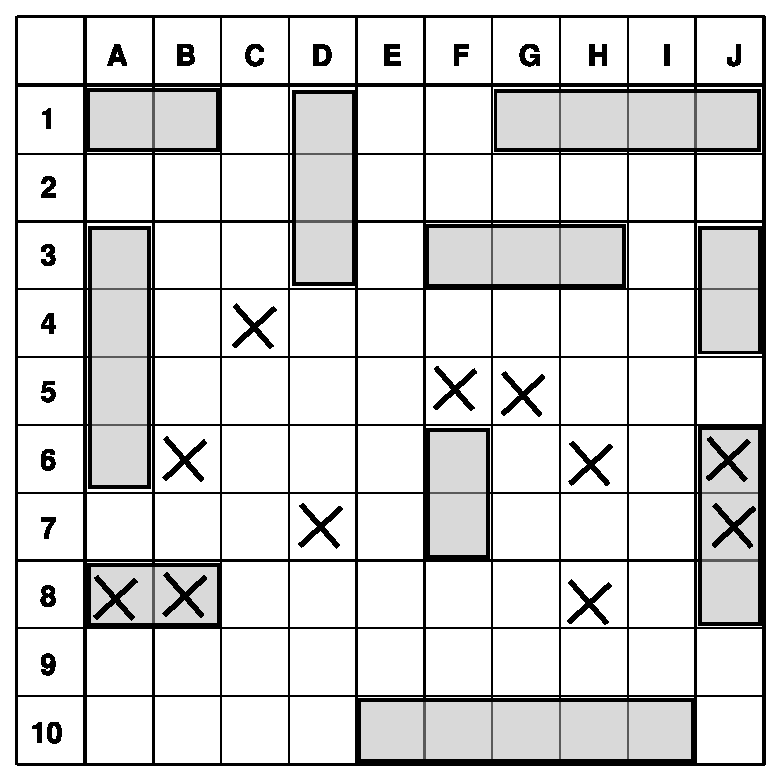
\includegraphics[width=\linewidth]{zeeslagbord.pdf}
		\end{column}
	\end{columns}
\end{frame}


\section{\texttt{pybattleships}}
\begin{frame}{\texttt{pybattleships}}
	\begin{itemize}
		\item Library voor abstractie van het spel: roep methoden aan en kijk wat eruit komt.
		\item Dwingt de spelregels af
		\item \texttt{Ship}, \texttt{Board}, \texttt{Game}
		\item \url{http://pybattleships.rtfd.io}
	\end{itemize}
\end{frame}

\subsection{Ship}
\begin{frame}{Ship}
	\begin{itemize}
		\item Bevat een schip
		\item Eigenschappen: \texttt{x}, \texttt{y}, \texttt{horizontal}, \texttt{size}
		\item Kan op geschoten worden, houdt bij of hij is geraakt / gezonken
	\end{itemize}
\end{frame}

\subsection{Board}
\begin{frame}{Board}
	\begin{itemize}
		\item Bevat 10 schepen
		\item Controleert of schepen niet overlappen
		\item Kan zien of je hebt verloren
		\item Geeft schoten door aan onderliggende Ships
	\end{itemize}
\end{frame}

\subsection{Game}
\begin{frame}{Game}
	\begin{itemize}
		\item Houdt speler aan zet bij, geeft schoten door aan onderliggende Boards
		\item Controleert of beide spelers geldig Board hebben voor start
	\end{itemize}
\end{frame}

\section{Aan de slag}
\begin{frame}{Aan de slag}
	De bot moet kunnen:
	\begin{itemize}
		\item Schieten (gebaseerd op vorige schoten en wat daaruit kwam)
		\item Verzinnen hoe zijn startbord eruit ziet
		\item (Mogelijk) zijn state aan het begin van het spel opzetten
	\end{itemize}

	Download het framework via: \url{https://github.com/maartenberg/chatbotworkshop} en zet je code in
	\texttt{bot\_behaviour.py}.
\end{frame}
\end{document}
